% !TeX root = surprises.tex

\selectlanguage{hebrew}


\chapter{משפט חמשת הצבעים}
\label{c.five}

מפות משתמשות בצבעים כדי להבחין בין איזור אחד לאחר על ידי צביעת איזורים סמוכים בצבעים שונים. ב-%
$1852$
\L{Francis Guthrie}
שם לב שניתן לצבוע את המחוזות באנגליה עם ארבעה צבעים בלבד. הטענה שארבעה צבעים מספיקים כדי לצבוע כל מפה מישורית נקראת 
\textbf{משפט ארבעת הצבעים}.
המשפט הוכח רק ב-%
$1976$
על ידי
\L{Kenneth Appel}
ו-%
\L{Wolfgang Haken}.
הם השתמשו במתמטיקה מתקדמת כדי להראות שאם יש דוגמה נגדית (מפה הדורשת יותר מארבעה בצבעים), אזי המפה קשורה לאחת מ-%
$1834$
תצורות. לצרוך בדיקת התצורות הללו הם השתמשו במחשב.

למרות שקשה מאוד להוכיח את משפט ארבעת הצבעים, ההוכחות של משפט חמשת הצבעים ומשפט ששת הצבעים פשוטות יחסית (סעיפים%
~\ref{s.six-color}, ~\ref{s.five-color}).
בדרך להוכיח את המשפטים נגדיר מפות מישוריות וגרפים מישוריים (סעיף%
~\ref{s.planar}),
נוכיח את הנוסחה של
\L{Euler}
(סעיף%
~\ref{s.euler})
ונראה שבגרף מישורי חייב להיות צומת שהמעלה שלו הוא פחות או שווה לחמש. בסעיף%
~\ref{s.nonplanar}
נשתמש בנוסחה של
\L{Euler}
כדי להראות ששני גרפים לא מישוריים.

ב-%
$1879$
\L{Alfred B. Kempe}
פירסם הוכחה של משפט ארבעת הצבעים וב-%
$1890$
\L{Percy J. Heawood}
הראה שההוכחה שגוייה. בסעיף%
~\ref{s.kempe}
נביא את ההוכחה השגוייה של 
\L{Kempe}
והדוגמה של
\L{Heawood}
שמפריך את ההוכחה.


\section{מפות מישוריות וגרפים מישוריים}\label{s.planar}

\begin{definition}
\textbf{מפה מישורית}
היא קבוצה של שטחים במישור עם גבולות משותפים.
\textbf{צביעה}
של מפה היא השמה של צבע לכל שטח כך שכל שטחים שיש להם גבולות  משותפים צבועים בצבעים שונים.
\end{definition}
\ref{f.five-planar-map-five}
מראה צביעה בחמישה צבעים של מפה מישורית עם עשרה שטחים.
\ref{f.five-planar-map-five}
מראה צביעה עם ארבעה צבעים של אותה מפה.
\begin{definition}
\textbf{גרף}
הוא קבוצה של 
\textbf{צמתים}
$V$
וקבוצה של 
\textbf{קשתות}
$E$,
כך שכל קשת מחבר לשני צמתים.

\textbf{גרף מישורי}
הוא גרף בו שתי קשתות לא חותכות אחת את השניה. בגרף מישורי קטע מהמישור התחום על ידי קבוצה של קשתות נקרא 
\textbf{שטח}.

\textbf{צביעה}
של גרף מישורי היא השמה של צבעים לצמתים כך ששני צמתים המחוברים על ידי קשת צבועים בצבעים שונים.
\end{definition}



\begin{figure}[tb]
\begin{center}
\begin{subfigure}{.4\textwidth}
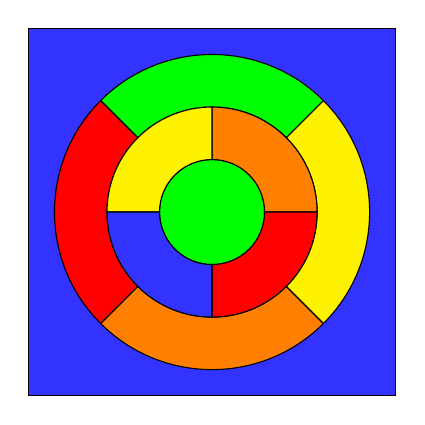
\begin{tikzpicture}[scale=.667]
\draw[fill=blue!80] (-3.5,-3.5) rectangle +(7,7);

\draw[fill=green] (0:1) 
  arc [start angle=0,  end angle=360, radius=1];

\draw[fill=green] (45:2) --
      (45:3)  arc[start angle=45,  end angle=135, radius=3] --
      (135:2) arc[start angle=135, end angle=45,  radius=2];
\draw[fill=orange] (-45:2) --
      (-45:3)  arc[start angle=-45,  end angle=-135, radius=3] --
      (-135:2) arc[start angle=-135, end angle=-45,  radius=2];
\draw[fill=yellow] (45:2) --
      (45:3)  arc[start angle=45,  end angle=-45, radius=3] --
      (-45:2) arc[start angle=-45, end angle=45,  radius=2];
\draw[fill=red] (135:2) --
      (135:3)  arc[start angle=135,  end angle=225, radius=3] --
      (225:2) arc[start angle=225, end angle=135,  radius=2];

\draw[fill=orange] (0:1) --
      (0:2)  arc[start angle=0,  end angle=90, radius=2] --
      (90:1) arc[start angle=90, end angle=0,  radius=1];
\draw[fill=red] (0:1) --
      (0:2)  arc[start angle=0,  end angle=-90, radius=2] --
      (-90:1) arc[start angle=-90, end angle=0,  radius=1];
\draw[fill=yellow] (90:1) --
      (90:2)  arc[start angle=90,  end angle=180, radius=2] --
      (180:1) arc[start angle=180, end angle=90,  radius=1];
\draw[fill=blue!80] (180:1) --
      (180:2)  arc[start angle=180,  end angle=270, radius=2] --
      (270:1) arc[start angle=270, end angle=180,  radius=1];
\end{tikzpicture}
\selectlanguage{hebrew}
\caption{צביעת מפה עם חמישה צבעים}\label{f.five-planar-map-five}
\end{subfigure}
\hspace{3em}
\begin{subfigure}{.4\textwidth}
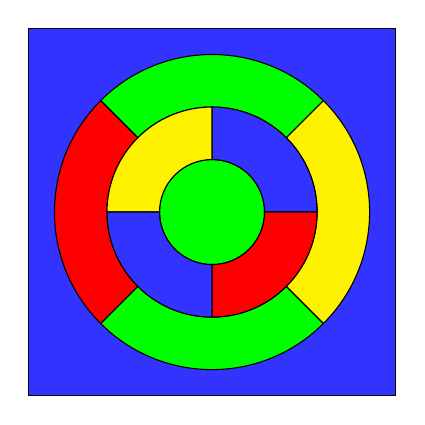
\begin{tikzpicture}[scale=.667]
\draw[fill=blue!80] (-3.5,-3.5) rectangle +(7,7);

\draw[fill=green] (0:1) 
  arc [start angle=0,  end angle=360, radius=1];

\draw[fill=green] (45:2) --
      (45:3)  arc[start angle=45,  end angle=135, radius=3] --
      (135:2) arc[start angle=135, end angle=45,  radius=2];
\draw[fill=green] (-45:2) --
      (-45:3)  arc[start angle=-45,  end angle=-135, radius=3] --
      (-135:2) arc[start angle=-135, end angle=-45,  radius=2];
\draw[fill=yellow] (45:2) --
      (45:3)  arc[start angle=45,  end angle=-45, radius=3] --
      (-45:2) arc[start angle=-45, end angle=45,  radius=2];
\draw[fill=red] (135:2) --
      (135:3)  arc[start angle=135,  end angle=225, radius=3] --
      (225:2) arc[start angle=225, end angle=135,  radius=2];

\draw[fill=blue!80] (0:1) --
      (0:2)  arc[start angle=0,  end angle=90, radius=2] --
      (90:1) arc[start angle=90, end angle=0,  radius=1];
\draw[fill=red] (0:1) --
      (0:2)  arc[start angle=0,  end angle=-90, radius=2] --
      (-90:1) arc[start angle=-90, end angle=0,  radius=1];
\draw[fill=yellow] (90:1) --
      (90:2)  arc[start angle=90,  end angle=180, radius=2] --
      (180:1) arc[start angle=180, end angle=90,  radius=1];
\draw[fill=blue!80] (180:1) --
      (180:2)  arc[start angle=180,  end angle=270, radius=2] --
      (270:1) arc[start angle=270, end angle=180,  radius=1];
\end{tikzpicture}
\selectlanguage{hebrew}
\caption{צביעת מפה עם ארבעה צבעים}\label{f.five-planar-map-four}
\end{subfigure}
\end{center}
\end{figure}
מפות וגרפים דואליים ונוח יותר לטפל בבעיות צביעה בגרפים ולא במפות.
\begin{theorem}
נתונה מפה מישורית, ניתן לבנות גרף מישורי כך שעבור כל צביעה של שטחים במפה קיימת צביעה של הצמתים בגרף, ולהיפך.
\end{theorem}

\begin{proof}
בנו צומת עבור כל שטח במפה ובנו קשת בין שני צמתים אם ורק אם קיים גבול בין שני השטחים.
\end{proof}
\begin{example}
\ref{f.five-planar-graph-map}
מראה את המפה המישורית מ-%
\ref{f.five-planar-map-four}
עם הצמתים המתאימים לכל השטחים. 
\ref{f.five-planar-graph-graph}
מראה גרף מישורי המתאים למפה.
\end{example}

\begin{figure}[tb]
\begin{center}
\begin{subfigure}{.45\textwidth}
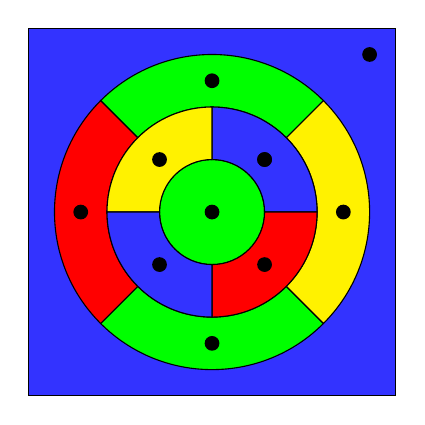
\begin{tikzpicture}[scale=.667]

\draw[fill=blue!80] (-3.5,-3.5) rectangle +(7,7);

\draw[fill=green] (0:1) 
  arc [start angle=0,  end angle=360, radius=1];

\draw[fill=green] (45:2) --
      (45:3)  arc[start angle=45,  end angle=135, radius=3] --
      (135:2) arc[start angle=135, end angle=45,  radius=2];
\draw[fill=green] (-45:2) --
      (-45:3)  arc[start angle=-45,end angle=-135,radius=3] --
      (-135:2) arc[start angle=-135, end angle=-45,  radius=2];
\draw[fill=yellow] (45:2) --
      (45:3)  arc[start angle=45,  end angle=-45, radius=3] --
      (-45:2) arc[start angle=-45, end angle=45,  radius=2];
\draw[fill=red] (135:2) --
      (135:3)  arc[start angle=135,  end angle=225, radius=3] --
      (225:2) arc[start angle=225, end angle=135,  radius=2];

\draw[fill=blue!80] (0:1) --
      (0:2)  arc[start angle=0,  end angle=90, radius=2] --
      (90:1) arc[start angle=90, end angle=0,  radius=1];
\draw[fill=red] (0:1) --
      (0:2)  arc[start angle=0,  end angle=-90, radius=2] --
      (-90:1) arc[start angle=-90, end angle=0,  radius=1];
\draw[fill=yellow] (90:1) --
      (90:2)  arc[start angle=90,  end angle=180, radius=2] --
      (180:1) arc[start angle=180, end angle=90,  radius=1];
\draw[fill=blue!80] (180:1) --
      (180:2)  arc[start angle=180,  end angle=270, radius=2] --
      (270:1) arc[start angle=270, end angle=180,  radius=1];

\foreach \x/\y/\name in {
    0/0/O,
    3/3/Z,
    1/1/E,-1/1/F,-1/-1/G,1/-1/H,
    0/2.5/A,2.5/0/B,0/-2.5/C,-2.5/0/D,
    } {
  \fill (\x,\y) coordinate(\name) circle(4pt);
}
\end{tikzpicture}
\selectlanguage{hebrew}
\caption{התאמת צמתים לשטחים\\
 במפה מישורית}
\label{f.five-planar-graph-map}
\end{subfigure}
\begin{subfigure}{.4\textwidth}
\hspace{2em}
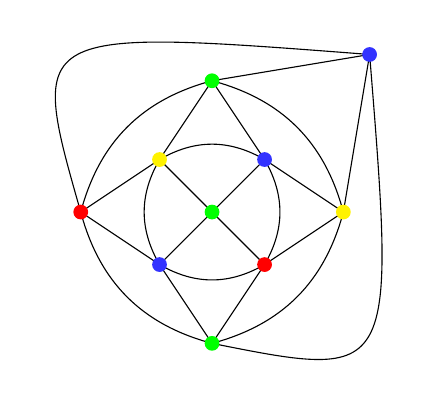
\begin{tikzpicture}[scale=.667]
\foreach \x/\y/\name in {
    0/0/O,
    3/3/Z,
    1/1/E,-1/1/F,-1/-1/G,1/-1/H,
    0/2.5/A,2.5/0/B,0/-2.5/C,-2.5/0/D,
    } {
  \coordinate(\name) at (\x,\y);
}

\draw (E) -- (O) -- (F);
\draw (G) -- (O) -- (H);
\draw (E) to [bend right=30] (F) to [bend right=30] (G) 
          to [bend right=30] (H) to [bend right=30] (E);
\draw (A) -- (E) -- (B) -- (H) -- (C) -- (G) -- (D) -- (F);
\draw (A) to [bend right=30] (D) to [bend right=30] (C) 
          to [bend right=30] (B) to [bend right=30] (A);

\draw (F) -- (A) -- (Z) -- (B);
\draw (C) .. controls (3.5,-3.2) .. (Z);
\draw (D) .. controls (-3.5,3.5) .. (Z);

\foreach \cl/\x/\y in {
    green/0cm/0cm,
    blue!80/3cm/3cm,
    blue!80/1cm/1cm,
    yellow/-1cm/1cm,
    blue!80/-1cm/-1cm,
    red/1cm/-1cm,
    green/0cm/2.5cm,
    yellow/2.5cm/0cm,
    green/0cm/-2.5cm,
    red/-2.5cm/0cm
    }
 \fill[\cl] (\x,\y) circle (4pt);
\end{tikzpicture}
\selectlanguage{hebrew}
\caption{התאמת גרף מישורי\\
למפה המישורית}
\label{f.five-planar-graph-graph}
\end{subfigure}
\end{center}
\end{figure}

ניתן להגביל את עצמנו לגרפים שהשטחים שלהם
\textbf{משולשיים}.

\begin{definition}
גרף הוא
\textbf{מתולת
\L{(triangular)}}
אם כל השטחים שלו חוסמים על ידי שלוש קשתות. ניתן 
\textbf{לתלת
\L{(triangulate)}}
גרף אם אפשר להוסיף קשתות כדי שהגרף יהי מתולת. אפשר גם להגיד שיש
\textbf{תילות
\L{(triangulation)}}
של הגרף.
\end{definition}
\begin{example}
השטחים של הגרף המישורי ב-%
\ref{f.five-planar-graph-graph}
מתולתים כי כל אחד חסום על ידי שלוש קשתות. הקשתות מעוגלות ולכן השטחים אינם משולשים, שהם מצולעים שצלעותיהם קטעי קו ישרים.
\end{example}
\begin{advanced}
משפט
\textbf{F\'{a}ry}
טוען שניתן להמר כל גרף מישורי מתולת לגרף מישורי שהקשתות שלו הם קטעי קו ישרים. מכאן, שללא הגבלת הכללית ניתן לנסח הוכחות רק עבור גרפים מישוריים שהשטחים שלהם משולשים.
\end{advanced}
\begin{example}
איור%
~\ref{f.five-triangular-graph}
(משמאל) מראה ריבוע שניתן לצבוע עם שני צבעים, אבל אם מתלתים אותו (במרכז) חייבים ארבעה צבעים. המטרה שלנו היא להוכיח שניתן לצבוע את כל הגרפים ב-%
$n$
צבעים (עבור
$n$
מסויים). אם ניתן לצבוע את הגרף המתולת עם 
$n$
צבעים, אפשר גם לצבוע את הגרף המקורי כי מחיקת הקשתות הנוספות לא מקלקל את הצביעה (ימין).
\end{example}

\begin{figure}[tb]
\begin{center}
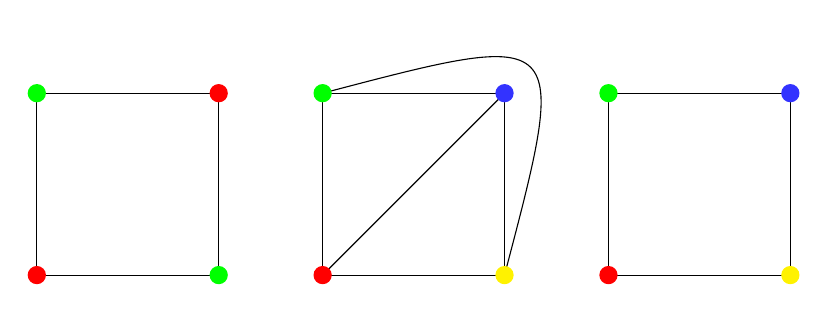
\begin{tikzpicture}[scale=.33]
\draw (-3.5,-3.5) rectangle +(7,7);
\fill[red] (-3.5,-3.5) circle(10pt);
\fill[green] (-3.5,3.5) circle(10pt);
\fill[green] (3.5,-3.5) circle(10pt);
\fill[red] (3.5,3.5) circle(10pt);
\begin{scope}[xshift=11cm]
\draw (-3.5,-3.5) -- (3.5,3.5);
\draw (-3.5,3.5) .. controls (6,6) .. (3.5,-3.5);
\draw (-3.5,-3.5) rectangle +(7,7);
\fill[red] (-3.5,-3.5) circle(10pt);
\fill[green] (-3.5,3.5) circle(10pt);
\fill[yellow] (3.5,-3.5) circle(10pt);
\fill[blue!80] (3.5,3.5) circle(10pt);
\end{scope}
\begin{scope}[xshift=22cm]
\draw (-3.5,-3.5) rectangle +(7,7);
\fill[red] (-3.5,-3.5) circle(10pt);
\fill[green] (-3.5,3.5) circle(10pt);
\fill[yellow] (3.5,-3.5) circle(10pt);
\fill[blue!80] (3.5,3.5) circle(10pt);
\end{scope}
\end{tikzpicture}
\selectlanguage{hebrew}
\caption{צביעת גרף מתולת}\label{f.five-triangular-graph}
\end{center}
\end{figure}

\section{הנוסחה של
\L{Euler}}\label{s.euler}

\begin{theorem}[\L{Euler}]\label{thm.euler}
יהי
$G$
גרף מישורי מקושר עם
$V$
צמתים,
$E$
קשתות ו-%
$F$
שטחים. אזי:
\[
V-E+F=2\,.
\]
\end{theorem}
\begin{proof}
באינדוקציה על מספר הקשתות. אם מספר הקשתות בגרף מישורי הוא אפס, קיים רק צומת אחד ושטח אחד כך ש-%
$1-0+1=2$.
אחרת, קיים לפחות קשת אחת
$e$
שמחבר שני צמתים
$v_1,v_2$.
נמחק את הקשת
$e$.

\textbf{מקרה 1:}
הגרף מפסיק להיות מקושר
(\ref{f.five-disconnected-removing}).
נשלב את
$v_1$
עם
$v_2$
(\ref{f.five-disconnected-merge}).
ל-%
$G'$
הגרף המישוי שנוצר פחות קשתות מ-%
$G$,
ולכן לפי הנחת האינדוקציה
$(V-1)-(E-1)+F=2$
כי יש גם צומת אחד פחות. נפשט ונקבל
$V-E+F=2$
עבור
$G$.

\begin{figure}[tb]
\begin{center}
\begin{subfigure}{.4\textwidth}
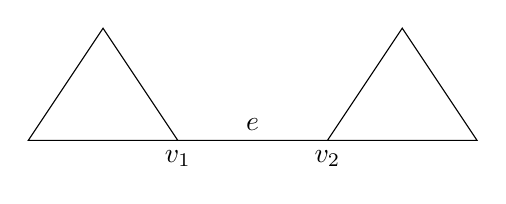
\begin{tikzpicture}[scale=.95]
\draw (2,0) -- (1,1.5) -- (0,0) -- (2,0) node[below] {$v_1$} -- node[above] {$e$} (4,0) node[below] {$v_2$} -- (6,0) -- (5,1.5) -- (4,0);
\end{tikzpicture}
\selectlanguage{hebrew}
\caption{הגרף לא קשור}\label{f.five-disconnected-removing}
\end{subfigure}
\hspace{3em}
\begin{subfigure}{.4\textwidth}
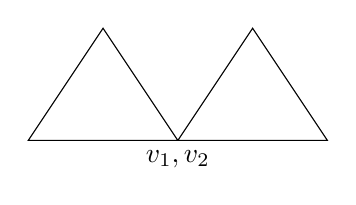
\begin{tikzpicture}[scale=.95]
\draw (2,0) -- (1,1.5) -- (0,0) -- (2,0) node[below] {$v_1,v_2$} -- (4,0) -- (3,1.5) -- (2,0);
\end{tikzpicture}
\selectlanguage{hebrew}
\caption{שילוב שני צמתים}\label{f.five-disconnected-merge}
\end{subfigure}
\end{center}
\end{figure}

\textbf{מקרה 2:}
הגרף נשאר מקושר
(\ref{f.five-connected-remains}).
לגרף הנוצר
$G'$
פחות קשתות מ-%
$G$
(\ref{f.five-connected-fewer}),
ולכן לפי הנחת האינדוקציה,
$V-(E-1)+(F-1)=2$
כי מחיקת קשת אחת מאחדת שני שטחים לאחד. נפשט ונקבל
$V-E+F=2$ 
עבור
$G$.
\end{proof}

\begin{figure}[tb]
\begin{center}
\begin{subfigure}{.4\textwidth}
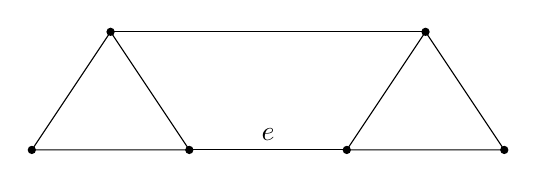
\begin{tikzpicture}
\foreach \x/\y in {0/0, 2/0, 1/1.5,4/0,6/0,5/1.5}
  \fill (\x,\y) circle (1.5pt);
\draw (2,0) -- (1,1.5) -- (0,0) -- (2,0);
\draw (2,0) -- node[above] {$e$} (4,0);
\draw (4,0) -- (6,0) -- (5,1.5) -- (4,0);
\draw (1,1.5) -- (5,1.5);
\end{tikzpicture}
\selectlanguage{hebrew}
\caption{הגרף נשאר קשור לאחר מחיקת קשת}\label{f.five-connected-remains}
\end{subfigure}
\hspace{3em}
\begin{subfigure}{.4\textwidth}
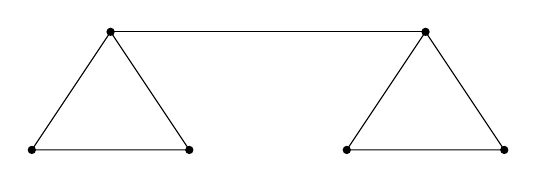
\begin{tikzpicture}
\foreach \x/\y in {0/0, 2/0, 1/1.5,4/0,6/0,5/1.5}
  \fill (\x,\y) circle (1.5pt);
\draw (2,0) -- (1,1.5) -- (0,0) -- (2,0);
\draw (4,0) -- (5,1.5) -- (6,0) -- cycle;
\draw (1,1.5) -- (5,1.5);
\end{tikzpicture}
\selectlanguage{hebrew}
\caption{הגרף קשור אבל עם פחות קשתות}
\label{f.five-connected-fewer}
\end{subfigure}
\end{center}
\end{figure}

\begin{theorem}\label{thm.edges}
יהי
$G$
גרף מישורי מקושר ומתולת. אזי
$E= 3V-6$.
\end{theorem}
\begin{proof}
כל שטח חסום על ידי שלוש קשתות כך ש-%
$E=3F/2$,
כי כל קשת נספר פעמיים, פעם אחת לכל שטח שהיא חוסמת. לפי נוסחת
\L{Euler}:
\begin{eqn}
E&=&V+F-2\\
E&=&V+2E/3-2\\
E&=&3V-6\,.
\end{eqn}
\end{proof}
\begin{example}
בגרף המישורי
\ref{f.five-planar-graph-graph}
יש
$10$
צמתים ו-%
$24= 3\cdot 10-6$
קשתות.
\end{example}
\begin{theorem}\label{thm.count}
יהי
$G$
גרף מישורי מקושר. אזי
$E\leq 3V-6$.
\end{theorem}
\begin{proof}
נתלת את
$G$
כדי לקבל
$G'$.
ב-%
$G'$, $E= 3V-6$
לפי משפט~%
\ref{thm.edges}.
נמחק קשתות מ-%
$G'$
כדי לקבל את
$G$.
מספר הצמתים לא משתנה כך ש-%
$E\leq 3V-6$.
\end{proof}

\begin{figure}[tb]
\begin{center}
\begin{subfigure}{.45\textwidth}
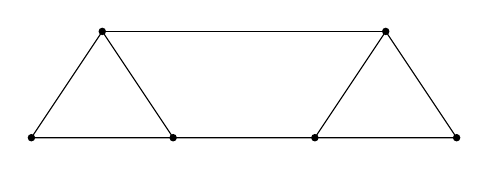
\begin{tikzpicture}[scale=.9]
\foreach \x/\y in {0/0, 2/0, 1/1.5,4/0,6/0,5/1.5}
  \fill (\x,\y) circle (1.5pt);
\draw (2,0) -- (1,1.5) -- (0,0) -- (2,0) -- (4,0) -- (6,0) -- (5,1.5) -- (4,0);
\draw (1,1.5) -- (5,1.5);
\node at (5.5,1) {};
\end{tikzpicture}
\selectlanguage{hebrew}
\caption{פחות קשתות מהחסם העליון}\label{f.five-fewer}
\end{subfigure}
\hspace{1em}
\begin{subfigure}{.45\textwidth}
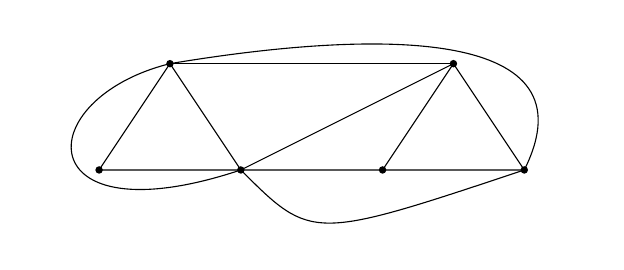
\begin{tikzpicture}[scale=.9]
\foreach \x/\y in {0/0, 2/0, 1/1.5,4/0,6/0,5/1.5}
  \fill (\x,\y) circle (1.5pt);
\draw (2,0) -- (1,1.5) -- (0,0) -- (2,0) -- (4,0) -- (6,0) -- (5,1.5) -- (4,0);
\draw (1,1.5) -- (5,1.5);
\draw (2,0) -- (5,1.5);
\draw (2,0) .. controls (-1,-1) and (-1,1) .. (1,1.5);
\draw (2,0) .. controls (3,-1) .. (6,0) .. controls (7,2) and (4,2) .. (1,1.5);
\end{tikzpicture}
\selectlanguage{hebrew}
\caption{בגרף מתולת מספר הקשתות מירבית}\label{f.five-upper-limit}
\end{subfigure}
\end{center}
\end{figure}
\begin{example}
לגרף ב-%
\ref{f.five-fewer}
$8$
קשתות ו-%
$6$
צמתים ולכן
$8< 3\cdot 6 - 6= 12$.
\ref{f.five-upper-limit}
מראה גרף מתולת עם
$6$
צמתים ו-%
$3\cdot 6 - 6= 12$
קשתות.
\end{example}

\section{גרפים שאינם מישוריים}
נסטה מעט מהסיפור כדי להראות איך ניתן להשתמש במשפטים 
\L{~\ref{thm.euler}}\label{s.nonplanar}
ו-%
\L{~\ref{thm.count}}
כדי להוכיח שגרפים מסויימים אינם מישוריים.

\begin{theorem}
$K_5$,
הגרף השלם עם חמישה צמתים, אינו מישורי 
(\ref{f.five-k5-failed}).
\end{theorem}
\begin{figure}[tb]
\begin{center}
\begin{subfigure}{.45\textwidth}
\begin{tikzpicture}[scale=.75]
\node (pentagon) [minimum size=4cm,regular polygon,regular polygon sides=5] at (0,0) {};
\draw (pentagon.corner 1) -- (pentagon.corner 2);
\draw (pentagon.corner 2) -- (pentagon.corner 3);
\draw (pentagon.corner 3) -- (pentagon.corner 4);
\draw (pentagon.corner 4) -- (pentagon.corner 5);
\draw (pentagon.corner 5) -- (pentagon.corner 1);
\draw (pentagon.corner 1) -- (pentagon.corner 3);
\draw (pentagon.corner 1) -- (pentagon.corner 4);
\draw (pentagon.corner 2) -- (pentagon.corner 4);
\draw (pentagon.corner 2) -- (pentagon.corner 5);
\draw (pentagon.corner 3) -- (pentagon.corner 5);
\node at (4,2) {};
\end{tikzpicture}
\selectlanguage{hebrew}
\caption{$K_5$
אינו מישורי}
\label{f.five-k5-failed}
\end{subfigure}
\hspace{1em}
\begin{subfigure}{.45\textwidth}
\begin{tikzpicture}[scale=.75]
\node (pentagon) [minimum size=4cm,regular polygon,regular polygon sides=5] at (0,0) {};
\draw (pentagon.corner 1) -- (pentagon.corner 2);
\draw (pentagon.corner 2) -- (pentagon.corner 3);
\draw (pentagon.corner 3) -- (pentagon.corner 4);
\draw (pentagon.corner 4) -- (pentagon.corner 5);
\draw (pentagon.corner 5) -- (pentagon.corner 1);
\draw (pentagon.corner 1) .. controls (-4,1) .. 
      (pentagon.corner 3);
\draw (pentagon.corner 1) .. controls (4,1) ..
      (pentagon.corner 4);
\draw (pentagon.corner 2) -- (pentagon.corner 4);
\draw (pentagon.corner 2) -- (pentagon.corner 5);
\draw (pentagon.corner 3) -- (pentagon.corner 5);
\draw[thick] (0,-.75) circle(5pt);
\end{tikzpicture}
\selectlanguage{hebrew}
\caption{$K_5$
אינו מישורי
}\label{f.k5}
\end{subfigure}
\end{center}
\end{figure}
\begin{proof}
עבור
$K_5$, $V=5$
ו-%
$E=10$.
לפי משפט%
~\ref{thm.count}
מספר הקשתות חייב להיות פחות או יותר מ-%
$3\cdot 5 -6=9$
ולכן הגרף לא מישורי.
\end{proof}
\begin{theorem}
$K_{3,3}$,
הגרף הדו-אזורי עם שלושה צמתים בכל איזור 
(\ref{f.five-k33}),
אינו מישורי.
\end{theorem}
\begin{figure}[tb]
\begin{center}
\begin{subfigure}{.4\textwidth}
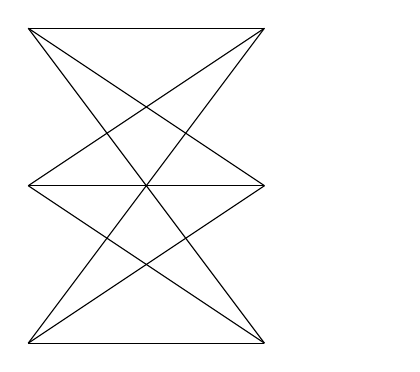
\begin{tikzpicture}[scale=1]
\draw (0,0) -- (3,0);
\draw (0,2) -- (3,2);
\draw (0,4) -- (3,4);
\draw (0,0) -- (3,2);
\draw (0,2) -- (3,4);
\draw (0,4) -- (3,0);
\draw (0,0) -- (3,4);
\draw (0,2) -- (3,0);
\draw (0,4) -- (3,2);
\node at (4.5,1) {};
\end{tikzpicture}
\selectlanguage{hebrew}
\caption{$K_{3,3}$ אינו מישורי}\label{f.five-k33}
\end{subfigure}
\hspace{3em}
\begin{subfigure}{.4\textwidth}
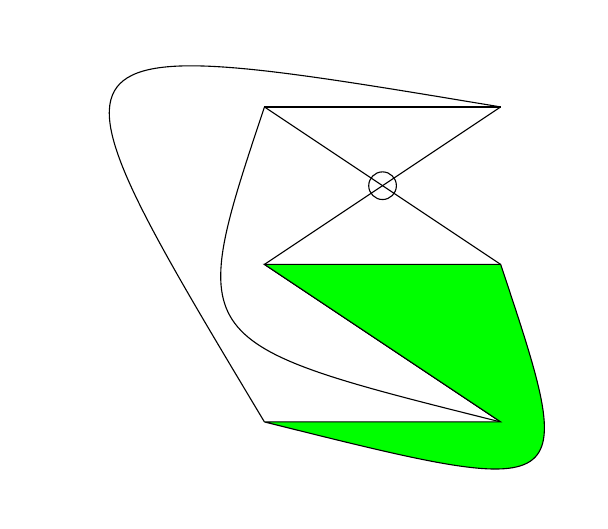
\begin{tikzpicture}
\draw (0,4) -- (3,4);
\draw (0,2) -- (3,4);
\draw (0,4) .. controls (-1,1) .. (3,0);
\draw (0,0) .. controls (-3,5) .. (3,4);
\draw (0,2) -- (3,0);
\draw (0,4) -- (3,2);
\draw[fill=green] (0,0) -- (3,0) -- (3,0) -- (0,2)  -- (3,2) .. controls (4,-1) .. (0,0);
\draw (1.5,3) circle(5pt);
\end{tikzpicture}
\selectlanguage{hebrew}
\caption{ניסיון כושל לצייר את
$K_{3,3}$
במישור}
\label{f.five-k33-failed}
\end{subfigure}
\end{center}
\end{figure}
\begin{proof}
$V=6$
ו-%
$E=9$.
לפי משפט%
~\ref{thm.euler},
אם
$K_{3,3}$
מישורי,
$F=E-V+2=9-6+2=5$.
אבל כל שטח תחום על ידי ארבע קשתות
\ref{f.five-k33-failed},
כך ש-
 ולכן
$E=4F/2=(4\cdot 5)/2\neq 9$.
\end{proof}

ב-%
$1930$
\L{Kazimierz Kuratowski}
הוכיח את הכיוון השני של המשפטים הללו: אם גרף אינו מישורי, אזי הוא מכיל (במובן מסויים) 
$K_5$
או
$K_{3,3}$.

%%%%%%%%%%%%%%%%%%%%%%%%%%%%%%%%%%%%%%%%%%%%%%%%%%%

\section{המעלה של הצמתים}\label{s.degrees}

\begin{definition}
$d(v)$,
\textbf{המעלה}
של צומת
$v$,
היא מספר הקשתות הנפגשות ב-%
$v$.
\end{definition}

\begin{example}
לגרף באיור%
~\ref{f.five-planar-graph-graph}
$8$
צמתים בתוך שתי הטבעות, כל אחד ממעלה
$5$.
המעלה של השטח החיצוני ושל השטח הפנימי הוא 
$4$.
לכן:
\[
\sum_{v\in V} d(v) = 5\cdot 8 + 4\cdot 2=48\,.
\]
נקבל את מספר הקשתות בגרף על ידי חלוקת סכום המעלות ב-%
$2$,
כי כל קשת נספרה פעמיים, פעם אחת עבור כל צומת שהיא נוגעת בו.
\end{example}
הכללת הטיעונים הללו מוכיחה:
\begin{theorem}\label{thm.degrees}
יהי
$d_i, i=1,2,3,\ldots,k$
מספרי הצמתים ממעלה
$i$
בגרף מישורי מקושר עם
$V$
צמתים ו-%
$E$ 
קשתות, כאשר
$k$
הוא המעלה הגבוהה ביותר של צומת ב-%
$V$.
אזי:
\[
\sum_{v\in V} d(v) =\sum_{i=1}^{k} i\cdot d_i=2E\,.
\]
\end{theorem}
\begin{theorem}\label{thm.degree5}
יהי
$G$
גרף מישורי מקושר עם
$E$
קשתות ו-%
$V$
צמתים, ויהי
$d_i,i=1,\ldots,k$
מספרי ההצמתים ממעלה
$i$,
כאשר
$k$
הוא המעלה הגבוהה ביותר של צומת ב-%
$V$.
אזי חייב להיות צומת
$v$
ב-%
$V$
כך ש-%
$d(v) \leq 5$.
\end{theorem}
\begin{proof}
\textbf{(1)}
ברור שאם יש 
$d_1$
צמתים ממעלה
$1$, $d_2$ 
צמתים ממעלה
$2$, \ldots, $d_k$
צמתים ממעלה
$k$, 
אזי
$V=\sum_{i=1}^{k}d_i$. 
מהמשפטים
\L{~\ref{thm.count}}
ו-%
\L{~\ref{thm.degrees}}
נקבל:
\[
\sum_{i=1}^{k} i\cdot d_i=2E\leq 2(3V-6) = 6V-12=6\sum_{i=1}^{k} d_i -12\,.
\]
מכאן ש:
\begin{eqn}
\sum_{i=1}^{k} i\cdot d_i \leq 6\sum_{i=1}^{k} d_i -12\\
\sum_{i=1}^{k} (6-i)d_i\geq 12\,.
\end{eqn}
$12>0$,
ולכן ל-%
$i$
אחד לפחות,
$6-i>0$
ועבור 
$i$
זה,
$i<6$. 
\end{proof}

\begin{proof}
\textbf{(2)}
נחשב את 
\textbf{הממוצע}
של המעלות של הצמתים שהוא סכום המעלות לחלק למספר הצמתים:
\[
d_{\textit{\footnotesize avg}}=\frac{\sum_{i=1}^{k} i\cdot d_i}{V}\,.
\]
אבל סכום המעלות הוא פעמיים מספר הקשתות ולפי משפט
\L{~\ref{thm.count}}:
\[
d_{\textit{\footnotesize avg}}=\frac{2E}{V}\leq \frac{6V-12}{V}=6-\frac{6}{V}<6\,.
\]
אם 
\textbf{הממוצע}
של המעלות הוא פחות משש חייב להיות צומת אחד לפחות ממעלה פחות משש.
\end{proof}

\begin{example}
סכום המעלות cברף באיור%
~\ref{f.five-planar-graph-graph}
הוא
$8\cdot 5 + 2\cdot 4=48$.
יש 
$10$
צמתים כך שממוצע המעלות שלו הוא
$48/10=4.8$
וחייב להיות צומת ממעלה 
$4$
או פחות.
\end{example}

\section{משפט ששת הבצעים}\label{s.six-color}

\begin{theorem}\label{thm.sixcolor}
כל גרף מישורי ניתן לצביעה בששה צבעים.
\end{theorem}

\begin{proof}
באינדוקציה על מספר הצמתים ב-%
$G$.
אם לגרף ששה צמתים או פחות, ברור שניתן לצבוע את הגרף בששה צבעים. עבור הצעד האינדוקטיבי, לפי משפט
\L{~\ref{thm.degree5}}
קיים צומת
$v$
ממעלה חמש או פחות. נמחק צומת
$v$
כדי לקבל את הגרף
$G'$.
לפי הנחת האינדוקציה ניתן לצבוע את
$G'$
עם ששה צבעים, אבל ל-%
$v$
חמישה שכנים לכל היותר שצבועים בחמישה צבעים לכל היותר
(\ref{f.five-six-five}),
כך שנשאר צבע ששי שניתן לצבוע בו את
$v$
(\ref{f.five-six-six}).
\end{proof}

\begin{figure}[tb]
\begin{center}
\begin{subfigure}{.4\textwidth}
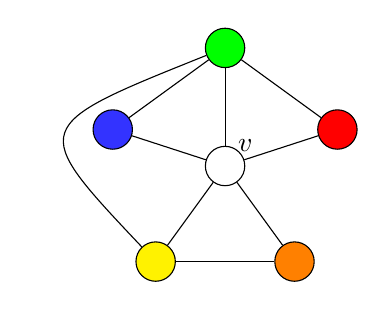
\begin{tikzpicture}[scale=.5,minimum size=5mm,inner sep=0pt]
\foreach \name/\color/\theta in
    {A/red/18,B/green/90,C/blue!80/162,D/yellow/234,E/orange/306}
  \node[circle,draw,fill=\color] (\name) at (\theta:3) {};
\node[circle,draw] (O) at (0,0) {};
\node[above right] at (O) {$v$};
\foreach \name in {A,B,C,D,E}
  \draw (O) -- (\name);
\foreach \i/\j in {A/B,B/C,D/E}
  \draw (\i) -- (\j);
\draw (B) .. controls (-5,1) .. (D);
\end{tikzpicture}
\selectlanguage{hebrew}
\caption{חמישה צבעים מספיקים
$v$}\label{f.five-six-five}
\end{subfigure}
\hspace{3em}
\begin{subfigure}{.4\textwidth}
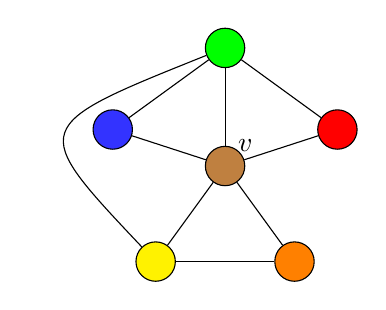
\begin{tikzpicture}[scale=.5,minimum size=5mm,inner sep=0pt]
\foreach \name/\color/\theta in
    {A/red/18,B/green/90,C/blue!80/162,D/yellow/234,E/orange/306}
  \node[circle,draw,fill=\color] (\name) at (\theta:3) {};
\node[circle,draw,fill=brown] (O) at (0,0) {};
\node[above right] at (O) {$v$};
\foreach \name in {A,B,C,D,E}
  \draw (O) -- (\name);
\foreach \i/\j in {A/B,B/C,D/E}
  \draw (\i) -- (\j);
\draw (B) .. controls (-5,1) .. (D);
\end{tikzpicture}
\selectlanguage{hebrew}
\caption{נצבע את
$v$
הצבע הששי}
\label{f.five-six-six}
\end{subfigure}
\end{center}
\end{figure}

\section{משפט חמשת הצבעים}\label{s.five-color}

\begin{definition}
יהי
$G$
גרף מישורי מקושר צבוע. 
$G'$
הוא
\textbf{שרשרת}
אם ורק אם
$G'$
הוא תת-גרף מקסימלי של
$G$
הצבוע בשני צבעים.%
\footnote{%
השרשרת נקראת גם
\textbf{שרשרת \L{Kempe}}
כי היא הוגדרה על ידי
\L{Alfred Kempe}
בהוכחה השגויה שלו למשפט ארבעת הצבעים.}
\end{definition}
\begin{theorem}\label{thm.fivecolor}
כל גרף מישורי 
$G$
ניתן לצבוע בחמישה צבעים.
\end{theorem}

\begin{proof}
באינדקציה על מספר הצמתים. אם ב-%
$G$
חמישה צמתים או פחות, ניתן לצבוע עם חמישה צבעים. עבור הצעד האינדוקטיבי, לפי משפט
\L{~\ref{thm.degree5}}
קיים צומת
$v$
ממעלה חמש או פחות. נמחק את הצומת
$v$
ונקבל את הגרף
$G'$.
לפי הנחת האינדוקציה, ניתן לצבוע את
$G'$
עם חמישה צבעים או פחות. ב-%
$G$,
אם המעלה של
$v$
היא פחות מחמש, או אם
$v_1,\ldots,v_5$,
השכנים של
$v$,
צבועים עם ארבעה צבעים או פחות, ניתן לצבוע את
$v$
עם הצבע החמישי. אחרת, הצמתים
$v_1,\ldots,v_5$
צבועים בצבעים שונים ב-%
$G'$
(איור%
~\ref{f.five-color-proof},
למעלה).
\begin{figure}[tb]
\begin{center}
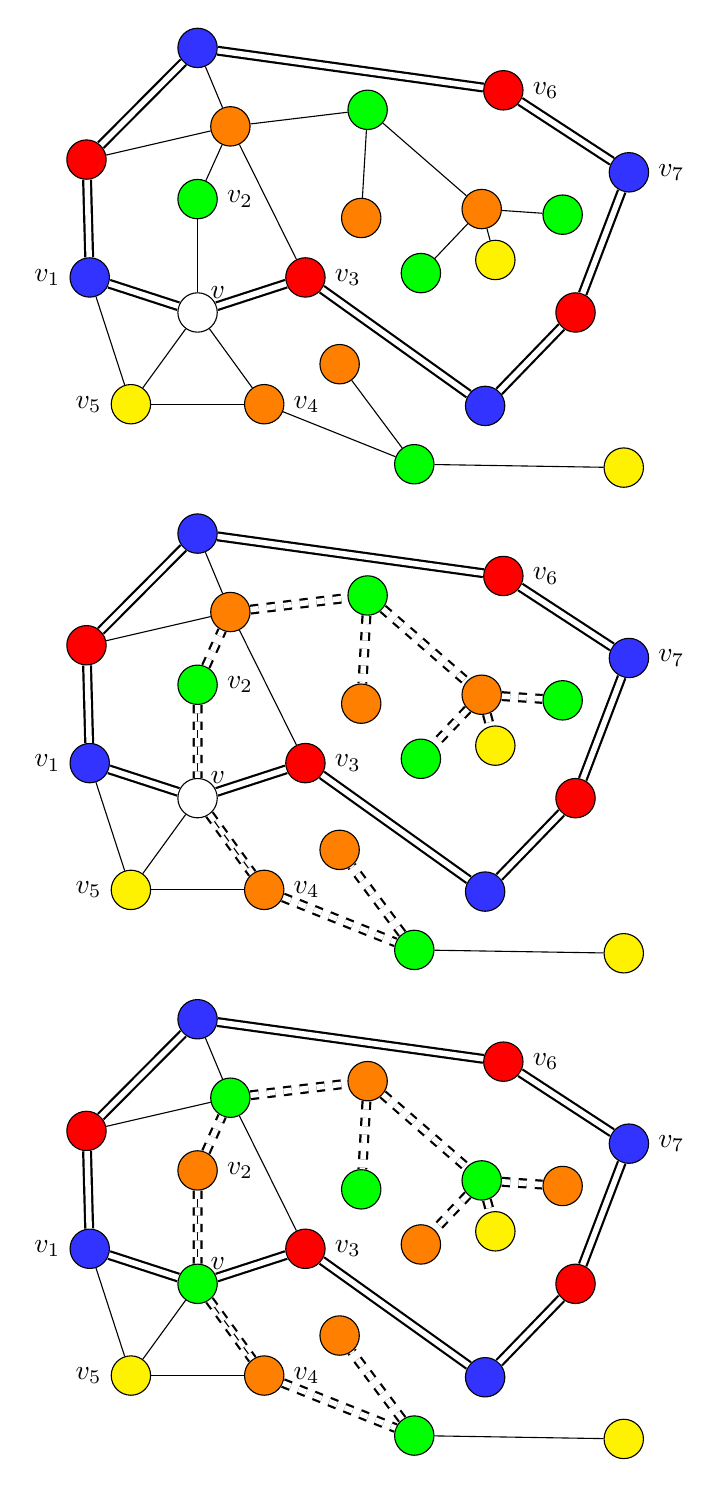
\begin{tikzpicture}[scale=.48,minimum size=5mm,inner sep=0pt]
\foreach \name/\color/\theta in
    {A/red/18,B/green/90,C/blue!80/162,D/yellow/234,E/orange/306}
  \node[circle,draw,fill=\color] (\name) at (\theta:3) {};
\node[circle,draw] (O) at (0,0) {};
\node[above right] at (O) {$v$};

\node[right,xshift=8pt] at (A) {$v_3$};
\node[right,xshift=8pt] at (B) {$v_2$};
\node[left,,xshift=-8pt] at (C) {$v_1$};
\node[left,,xshift=-8pt] at (D) {$v_5$};
\node[right,xshift=8pt] at (E) {$v_4$};

\foreach \name in {A,B,C,D,E}
  \draw (O) -- (\name);
  
\node[circle,draw,fill=red]  (X1) at (126:5) {};
\node[circle,draw,fill=blue!80] (X2) at (90:7)  {};
\node[circle,draw,fill=red]  (X3) at (36:10) {};
\node[right,xshift=8pt] at (X3) {$v_6$};
\node[circle,draw,fill=blue!80] (X4) at (18:12) {};
\node[right,xshift=8pt] at (X4) {$v_7$};
\node[circle,draw,fill=red]  (X5) at (0:10) {};
\node[circle,draw,fill=blue!80] (X6) at (-18:8) {};
\draw[thick,double distance=2pt] (C)  -- (X1);
\draw[thick,double distance=2pt] (X1) -- (X2);
\draw[thick,double distance=2pt] (X2) -- (X3);
\draw[thick,double distance=2pt] (X3) -- (X4);
\draw[thick,double distance=2pt] (X4) -- (X5);
\draw[thick,double distance=2pt] (X5) -- (X6);
\draw[thick,double distance=2pt] (X6) -- (A);
\draw[thick,double distance=2pt] (A) -- (O) -- (C);

\node[circle,draw,fill=orange]  (Y1)  at (80:5) {};
\node[circle,draw,fill=green]   (Y2)  at (50:7)  {};
\node[circle,draw,fill=orange]  (Y3A) at (20:8) {};
\node[circle,draw,fill=orange]  (Y3B) at (30:5) {};
\node[circle,draw,fill=green]   (Y4A) at (10:6) {};
\node[circle,draw,fill=yellow]  (Y4B) at (10:8) {};
\node[circle,draw,fill=green]   (Y4C) at (15:10) {};
\node[circle,draw,fill=green]   (Y5)  at (-35:7) {};
\node[circle,draw,fill=yellow]  (Y6A) at (-20:12) {};
\node[circle,draw,fill=orange]  (Y6B) at (-20:4) {};
\draw (B)  -- (Y1);
\draw (Y1) -- (Y2);
\draw (Y2) -- (Y3A);
\draw (Y2) -- (Y3B);
\draw (Y3A) -- (Y4A);
\draw (Y3A) -- (Y4B);
\draw (Y3A) -- (Y4C);
\draw (E)  -- (Y5);
\draw (Y5) -- (Y6A);
\draw (Y5) -- (Y6B);
\draw (A) -- (Y1);
\draw (X2) -- (Y1);
\draw (X1) -- (Y1);
\draw (D) -- (E);
\draw (D) -- (C);

\begin{scope}[yshift=-12.85cm]
\foreach \name/\color/\theta in
    {A/red/18,B/green/90,C/blue!80/162,D/yellow/234,E/orange/306}
  \node[circle,draw,fill=\color] (\name) at (\theta:3) {};
\node[circle,draw] (O) at (0,0) {};
\node[above right] at (O) {$v$};

\node[right,xshift=8pt] at (A) {$v_3$};
\node[right,xshift=8pt] at (B) {$v_2$};
\node[left,,xshift=-8pt] at (C) {$v_1$};
\node[left,,xshift=-8pt] at (D) {$v_5$};
\node[right,xshift=8pt] at (E) {$v_4$};

\foreach \name in {A,B,C,D,E}
  \draw (O) -- (\name);
  
\node[circle,draw,fill=red]  (X1) at (126:5) {};
\node[circle,draw,fill=blue!80] (X2) at (90:7)  {};
\node[circle,draw,fill=red]  (X3) at (36:10) {};
\node[circle,draw,fill=blue!80] (X4) at (18:12) {};
\node[circle,draw,fill=red]  (X5) at (0:10) {};
\node[circle,draw,fill=blue!80] (X6) at (-18:8) {};

\draw[thick,double distance=2pt] (C)  -- (X1);
\draw[thick,double distance=2pt] (X1) -- (X2);
\draw[thick,double distance=2pt] (X2) -- (X3);
\draw[thick,double distance=2pt] (X3) -- (X4);
\draw[thick,double distance=2pt] (X4) -- (X5);
\draw[thick,double distance=2pt] (X5) -- (X6);
\draw[thick,double distance=2pt] (X6) -- (A);
\draw[thick,double distance=2pt] (A) -- (O) -- (C);

\node[circle,draw,fill=orange]  (Y1)  at (80:5) {};
\node[circle,draw,fill=green]   (Y2)  at (50:7)  {};
\node[circle,draw,fill=orange]  (Y3A) at (20:8) {};
\node[circle,draw,fill=orange]  (Y3B) at (30:5) {};
\node[circle,draw,fill=green]   (Y4A) at (10:6) {};
\node[circle,draw,fill=yellow]   (Y4B) at (10:8) {};
\node[circle,draw,fill=green]   (Y4C) at (15:10) {};
\node[circle,draw,fill=green]   (Y5)  at (-35:7) {};
\node[circle,draw,fill=yellow]  (Y6A) at (-20:12) {};
\node[circle,draw,fill=orange]  (Y6B) at (-20:4) {};
\draw[thick,dashed,double distance=2pt] (B)  -- (O) -- (E);
\draw[thick,dashed,double distance=2pt] (B)  -- (Y1);
\draw[thick,dashed,double distance=2pt] (Y1) -- (Y2);
\draw[thick,dashed,double distance=2pt] (Y2) -- (Y3A);
\draw[thick,dashed,double distance=2pt] (Y2) -- (Y3B);
\draw[thick,dashed,double distance=2pt] (Y3A) -- (Y4A);
\draw[thick,dashed,double distance=2pt] (Y3A) -- (Y4B);
\draw[thick,dashed,double distance=2pt] (Y3A) -- (Y4C);
\draw[thick,dashed,double distance=2pt] (E)  -- (Y5);
\draw[thick,dashed,double distance=2pt] (Y5) -- (Y6B);
\draw (Y5) -- (Y6A);
\draw (A) -- (Y1);
\draw (X2) -- (Y1);
\draw (X1) -- (Y1);
\draw (D) -- (E);
\draw (D) -- (C);
\node[right,xshift=8pt] at (X3) {$v_6$};
\node[right,xshift=8pt] at (X4) {$v_7$};
\end{scope}

\begin{scope}[yshift=-25.7cm]
\foreach \name/\color/\theta in
    {A/red/18,B/orange/90,C/blue!80/162,D/yellow/234,E/orange/306}
  \node[circle,draw,fill=\color] (\name) at (\theta:3) {};
\node[circle,draw,fill=green] (O) at (0,0) {};
\node[above right] at (O) {$v$};

\node[right,xshift=8pt] at (A) {$v_3$};
\node[right,xshift=8pt] at (B) {$v_2$};
\node[left,,xshift=-8pt] at (C) {$v_1$};
\node[left,,xshift=-8pt] at (D) {$v_5$};
\node[right,xshift=8pt] at (E) {$v_4$};

\foreach \name in {A,B,C,D,E}
  \draw (O) -- (\name);
  
\node[circle,draw,fill=red]  (X1) at (126:5) {};
\node[circle,draw,fill=blue!80] (X2) at (90:7)  {};
\node[circle,draw,fill=red]  (X3) at (36:10) {};
\node[circle,draw,fill=blue!80] (X4) at (18:12) {};
\node[circle,draw,fill=red]  (X5) at (0:10) {};
\node[circle,draw,fill=blue!80] (X6) at (-18:8) {};

\draw[thick,double distance=2pt] (C)  -- (X1);
\draw[thick,double distance=2pt] (X1) -- (X2);
\draw[thick,double distance=2pt] (X2) -- (X3);
\draw[thick,double distance=2pt] (X3) -- (X4);
\draw[thick,double distance=2pt] (X4) -- (X5);
\draw[thick,double distance=2pt] (X5) -- (X6);
\draw[thick,double distance=2pt] (X6) -- (A);
\draw[thick,double distance=2pt] (A) -- (O) -- (C);

\node[circle,draw,fill=green]  (Y1)  at (80:5) {};
\node[circle,draw,fill=orange]   (Y2)  at (50:7)  {};
\node[circle,draw,fill=green]  (Y3A) at (20:8) {};
\node[circle,draw,fill=green]  (Y3B) at (30:5) {};
\node[circle,draw,fill=orange]   (Y4A) at (10:6) {};
\node[circle,draw,fill=yellow]   (Y4B) at (10:8) {};
\node[circle,draw,fill=orange]   (Y4C) at (15:10) {};
\node[circle,draw,fill=green]   (Y5)  at (-35:7) {};
\node[circle,draw,fill=yellow]  (Y6A) at (-20:12) {};
\node[circle,draw,fill=orange]  (Y6B) at (-20:4) {};

\draw[thick,dashed,double distance=2pt] (B)  -- (O) -- (E);
\draw[thick,dashed,double distance=2pt] (B)  -- (Y1);
\draw[thick,dashed,double distance=2pt] (Y1) -- (Y2);
\draw[thick,dashed,double distance=2pt] (Y2) -- (Y3A);
\draw[thick,dashed,double distance=2pt] (Y2) -- (Y3B);
\draw[thick,dashed,double distance=2pt] (Y3A) -- (Y4A);
\draw[thick,dashed,double distance=2pt] (Y3A) -- (Y4B);
\draw[thick,dashed,double distance=2pt] (Y3A) -- (Y4C);
\draw[thick,dashed,double distance=2pt] (E)  -- (Y5);
\draw[thick,dashed,double distance=2pt] (Y5) -- (Y6B);


\draw (Y5) -- (Y6A);
\draw (A) -- (Y1);
\draw (X2) -- (Y1);
\draw (X1) -- (Y1);
\draw (D) -- (E);
\draw (D) -- (C);
\node[right,xshift=8pt] at (X3) {$v_6$};
\node[right,xshift=8pt] at (X4) {$v_7$};
\end{scope}
\end{tikzpicture}
\end{center}
\selectlanguage{hebrew}
\caption{הוכחת משפט חמשת הצבעים}\label{f.five-color-proof}
\end{figure}

הצומת
$v_1$
צבוע בכחול והצומת 
$v_3$
צבוע באדום. אם
$v_1,v_3$
לא קשורים במסלול כחול-אדום (למשל, אם הקשת 
$\overline{v_6v_7}$
לא היה קיים), ניתן להחליף את הצבעים על המסלול מ-%
$v_1$
ל-%
$v_6$
ולצבוע את 
$v$
בכחול. אחרת, ניקח את השרשרת הכחול-אדום שמכילה את
$v_1,v_3$
ונוסיף את
$v$
והקשתות
$\overline{vv_1},\overline{vv_3}$.
נקבל מסלול סגור
$P$
(המסומן בקו כפול) שמחלק את המישור לשטח "פנימי" ולשטח "חיצוני" (איור%
~\ref{f.five-color-proof}, אמצע).

כעת נתבונן בצומת
$v_2$
הצבוע ירוק ובצומת
$v_4$
הצבוע כתום. הצמתים הללו 
\textbf{אינם}
יכולים להיות בשרשרת ירוק-כתום אחת, כי 
$v_2$
נמצא 
\textbf{בתוך}
$P$
ו-%
$v_4$
נמצא
\textbf{מחוץ}
ל-%
$P$,
ולכן כל מסלול המחבר אותם חייב לחתוך את
$P$,
וזה סותר את ההנחה שהגרף מישורי. לכן הם חייבים להיות בתוך שתי שרשראות ירוק-כתום 
\textbf{לא קשורות}
(מסומנות בקו מקווקוו כפול באיור
~\ref{f.five-color-proof}, באמצע).
נחליף את שני ההצבעים בשרשרת המכילה את
$v_2$
ואז אפשר לצבוע את 
$v$
בירוק כדי לקבל צביעה עם חמישה צבעים של 
$G$
(איור%
~\ref{f.five-color-proof}, למטה).
\end{proof}

%%%%%%%%%%%%%%%%%%%%%%%%%%%%%%%%%%%%%%%%%%%%%%%%%%%%%%%%%%%

\begin{advanced}
הטענה שמסלול רציף מתוך עקומה רציפה סגורה 
$P$
אל מחוץ ל-%
$P$
חייב לחתוך את
$P$
היא ה-%
\L{\textbf{Jordan Curve Theorem}}.
המשפט ברור אינטואיטיבית אבל קשה להוכחה.
\end{advanced}

%%%%%%%%%%%%%%%%%%%%%%%%%%%%%%%%%%%%%%%%%%%%%%%%%%%%%%%%%%%

\section{ההוכחה השגויה של
\L{Kempe}
לבעיית ארבע הצבעים}
\label{s.kempe}

\begin{proof}
\textbf{(שגויה)}
טענת הבסיס רוב ההוכחה זהה להוכחה של משפט חמשת הצבעים. המקרה החדש שיש לקחת בחשבון הוא צומת 
$v$
עם חמישה שכנים שלפי ההנחה האינדוקטיבית ניתן לצבוע אותם
\textbf{בארבעה}
צבעים לאחר מחיקת הצומת
$v$.

ב-%
\ref{f.five-kempe1}
קיימים שני צמתים
$v_2,v_5$
הצבועים בכחול. נתבונן בשרשרת הכחול-ירוק המכילה את 
$v_2$
ובשרשרת הכחול-צהוב המכילה את
$v_5$.
השרשרת הכחול-ירוק נמצאת מתוך המסלול הסגור המוגדר על ידי השרשרת האדום-צהוב שמכילה את
$v_1,v_3$
(מסומן בקו כפול), והשרשרת הכחול-צהוב נמצאת בתוך המסלול הסגור המוגדר על ידי השרשרת האדום-ירוק המכילה את
$v_1,v_4$
(מסומן בקו כפול מקווקוו).

נחליף את הצבעים בשרשרת הכחול-ירוק ובשרשרת הכחול-צהוב 
(\ref{f.five-kempe1-exchange}).
השכנים של
$v$
צבועים בשלושה צבעים, אדום, ירוק צהוב, וניתן לצבוע את
$v$
בכחול.
\end{proof}


\begin{figure}[tb]
\begin{center}
\begin{subfigure}{.4\textwidth}
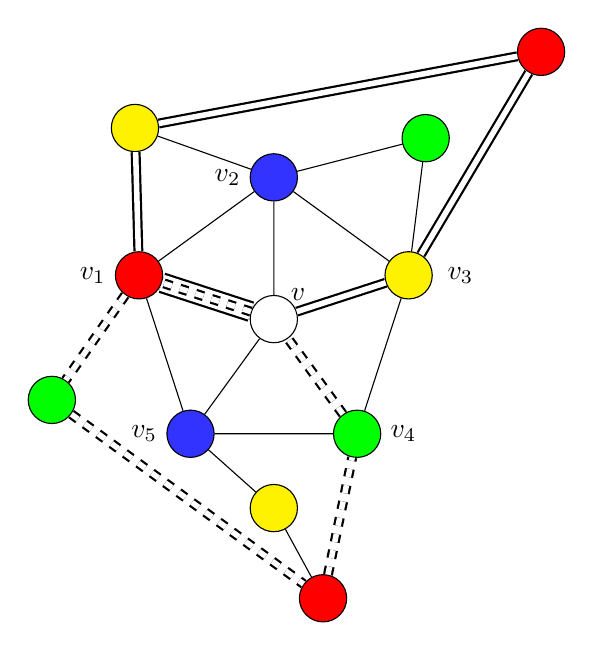
\begin{tikzpicture}[scale=.6,minimum size=6mm,inner sep=0pt]

% Draw center node and adjacent nodes
\foreach \name/\color/\theta in
    {A/yellow/18,B/blue!80/90,C/red/162,D/blue!80/234,E/green/306}
  \node[circle,draw,fill=\color] (\name) at (\theta:3) {};
\node[circle,draw] (O) at (0,0) {};
\node[above right]     at (O) {$v$};

\node[right,xshift=10pt] at (A) {$v_3$};
\node[left,xshift=-8pt]  at (B) {$v_2$};
\node[left,xshift=-8pt]  at (C) {$v_1$};
\node[left,xshift=-8pt]  at (D) {$v_5$};
\node[right,xshift=8pt]  at (E) {$v_4$};

% Draw red-yellow path
\node[circle,draw,fill=yellow]  (X1) at (126:5) {};
\node[circle,draw,fill=red] (X2) at (45:8)  {};

\draw[thick,double distance=2pt] 
  (C) -- (X1) -- (X2) -- (A) -- (O);
\draw[thick,double distance=6pt] (O) -- (C);

% Draw blue-green nodes within red-yellow path
\node[circle,draw,fill=green] (Y1)  at (50:5) {};

% Draw red-green path
\node[circle,draw,fill=green] (Z1)  at (-160:5) {};
\node[circle,draw,fill=red]   (Z2)  at (-80:6)  {};

%\draw[thick,dashed,double distance=6pt] (O) -- (C);
\draw[thick,dashed,double distance=2pt] 
  (O) -- (C) -- (Z1) -- (Z2) -- (E) -- (O);

% Draw blue-yellow nodes within red-green path
\node[circle,draw,fill=yellow]   (U1)  at (-90:4)  {};

% Connect adjacent nodes not in paths
\draw (X1) -- (B) -- (Y1) -- (A) -- (B) -- 
      (C) -- (D) -- (E) -- (A);
\draw (Z2) -- (U1) -- (D) -- (O) -- (B);

\end{tikzpicture}
\selectlanguage{hebrew}
\caption{שרשארות
\L{Kempe}
ירוק-כחול וכחול-צהוב}
\label{f.five-kempe1}
\end{subfigure}
\hspace{3em}
\begin{subfigure}{.4\textwidth}
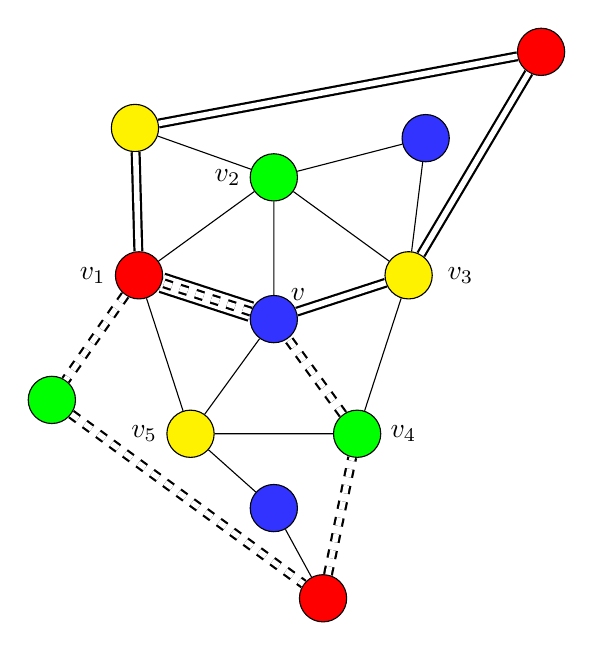
\begin{tikzpicture}[scale=.6,minimum size=6mm,inner sep=0pt]
% Draw center node and adjacent nodes
\foreach \name/\color/\theta in
    {A/yellow/18,B/green/90,C/red/162,D/yellow/234,E/green/306}
  \node[circle,draw,fill=\color] (\name) at (\theta:3) {};
\node[circle,draw,fill=blue!80] (O) at (0,0) {};
\node[above right]     at (O) {$v$};

\node[right,xshift=10pt] at (A) {$v_3$};
\node[left,xshift=-8pt]  at (B) {$v_2$};
\node[left,xshift=-8pt]  at (C) {$v_1$};
\node[left,xshift=-8pt]  at (D) {$v_5$};
\node[right,xshift=8pt]  at (E) {$v_4$};

% Draw red-yellow path
\node[circle,draw,fill=yellow]  (X1) at (126:5) {};
\node[circle,draw,fill=red] (X2) at (45:8)  {};

\draw[thick,double distance=2pt] 
  (C) -- (X1) -- (X2) -- (A) -- (O);
\draw[thick,double distance=6pt] (O) -- (C);

% Draw blue-green nodes within red-yellow path
\node[circle,draw,fill=blue!80] (Y1)  at (50:5) {};

% Draw red-green path
\node[circle,draw,fill=green] (Z1)  at (-160:5) {};
\node[circle,draw,fill=red]   (Z2)  at (-80:6)  {};

\draw[thick,dashed,double distance=2pt] 
  (O) -- (C) -- (Z1) -- (Z2) -- (E) -- (O);

% Draw blue-yellow nodes within red-green path
\node[circle,draw,fill=blue!80]   (U1)  at (-90:4)  {};

% Connect adjacent nodes not in paths
\draw (X1) -- (B) -- (Y1) -- (A) -- (B) -- 
      (C) -- (D) -- (E) -- (A);
\draw (Z2) -- (U1) -- (D) -- (O) -- (B);
\end{tikzpicture}
\selectlanguage{hebrew}
\caption{החלפת הצבעים של שתי שרשראות
\L{Kempe}}\label{f.five-kempe1-exchange}
\end{subfigure}
\end{center}
\end{figure}

\L{Heawood}
שם לב שיש אפשרות שלמסלולים הסגורים המוגדרים על ידי השרשראות האדום-צהוב והאדום-ירוק יש צמתים אדומים משותפים
($v_1,v_8$
ב-%
\ref{f.five-kempe2}).
כאשר מחליפים צבעים בשרשראות הכחול-ירוק והכחול-צהוב, יש אפשרות שיהיו צמתים צבועים בכחול הקשורים בקשת
(\ref{f.five-kempe2-share}),
כך שהצביעה כבר לא חוקית.
\begin{figure}[tb]
\begin{center}
\begin{subfigure}{.4\textwidth}
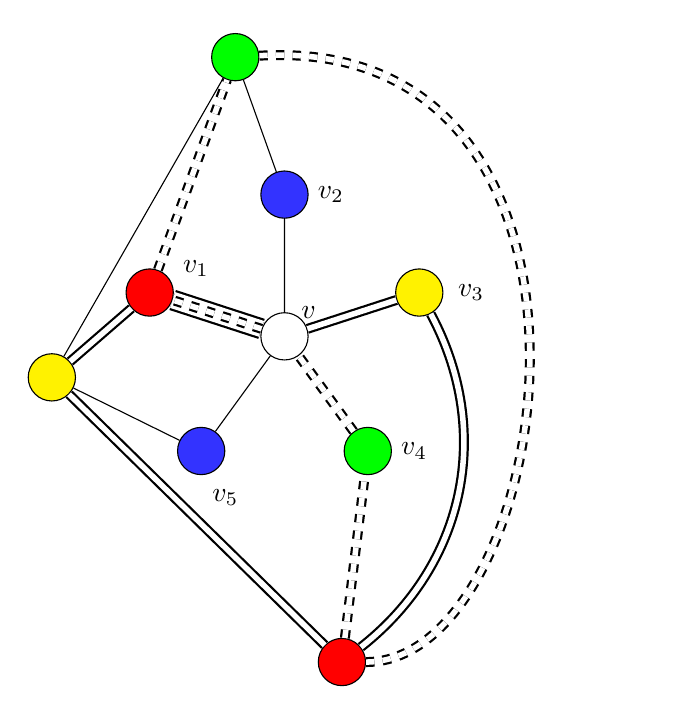
\begin{tikzpicture}[scale=.6,minimum size=6mm,inner sep=0pt]

% Draw center node and adjacent nodes
\foreach \name/\color/\theta in
    {A/yellow/18,B/blue!80/90,C/red/162,D/blue!80/234,E/green/306}
  \node[circle,draw,fill=\color] (\name) at (\theta:3) {};
\node[circle,draw] (O) at (0,0) {};
\node[above right]     at (O) {$v$};

\node[right,xshift=10pt] at (A) {$v_3$};
\node[right,xshift=8pt]  at (B) {$v_2$};
\node[above right,xshift=8pt]  at (C) {$v_1$};
\node[below right,yshift=-8pt] at (D) {$v_5$};
\node[right,xshift=8pt]  at (E) {$v_4$};

% Draw red-yellow path
\node[circle,draw,fill=yellow] (X1) at (-170:5) {};
\node[circle,draw,fill=red]    (X2) at (-80:7)  {};

\draw[thick,double distance=2pt] (A) -- (O);
\draw[thick,double distance=6pt] (O) -- (C);
\draw[thick,double distance=2pt] (C) --(X1) -- (X2);
\draw[thick,double distance=2pt,bend right=40] (X2) to (A);

% Draw red-green path
\node[circle,draw,fill=green] (Y1) at (100:6)  {};

\draw[dashed,thick,double distance=2pt] (O) -- (C) -- (Y1);
\draw[dashed,thick,double distance=2pt] 
  (Y1) .. controls (40:10) and (-50:9) .. (X2);
\draw[dashed,thick,double distance=2pt] (X2) -- (E) -- (O);

% Draw adjacent nodes
\draw (X1) -- (D) -- (O) -- (B) -- (Y1) -- (X1);

\end{tikzpicture}
\caption{לשרשארות אדום-צהוב ואדום-ירוק צמתים אדומים משותפים}
\label{f.five-kempe2}
\end{subfigure}
\hspace{3em}
\begin{subfigure}{.4\textwidth}
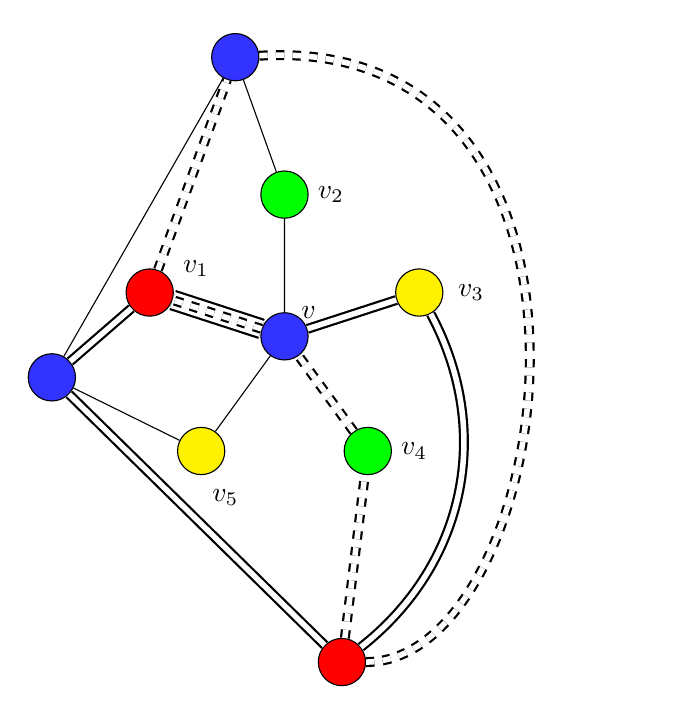
\begin{tikzpicture}[scale=.6,minimum size=6mm,inner sep=0pt]

% Draw center node and adjacent nodes
\foreach \name/\color/\theta in
    {A/yellow/18,B/green/90,C/red/162,D/yellow/234,E/green/306}
  \node[circle,draw,fill=\color] (\name) at (\theta:3) {};
\node[circle,draw,fill=blue!80] (O) at (0,0) {};
\node[above right]     at (O) {$v$};

\node[right,xshift=10pt] at (A) {$v_3$};
\node[right,xshift=8pt]  at (B) {$v_2$};
\node[above right,xshift=8pt]  at (C) {$v_1$};
\node[below right,yshift=-8pt] at (D) {$v_5$};
\node[right,xshift=8pt]  at (E) {$v_4$};


% Draw red-yellow path
\node[circle,draw,fill=blue!80] (X1) at (-170:5) {};
\node[circle,draw,fill=red]  (X2) at (-80:7)  {};

\draw[thick,double distance=2pt] (A) -- (O);
\draw[thick,double distance=6pt] (O) -- (C);
\draw[thick,double distance=2pt] (C) --(X1) -- (X2);
\draw[thick,double distance=2pt,bend right=40] (X2) to (A);

% Draw red-green path
\node[circle,draw,fill=blue!80] (Y1) at (100:6)  {};

\draw[dashed,thick,double distance=2pt] (O) -- (C) -- (Y1);
\draw[dashed,thick,double distance=2pt] 
  (Y1) .. controls (40:10) and (-50:9) .. (X2);
\draw[dashed,thick,double distance=2pt] (X2) -- (E) -- (O);

% Draw adjacent nodes
\draw (X1) -- (D) -- (O) -- (B) -- (Y1) -- (X1);
\end{tikzpicture}
\selectlanguage{hebrew}
\caption{החלפת הצבעים גורמת לצמתי הכחולים להיות קשורים}\label{f.five-kempe2-share}
\end{subfigure}
\end{center}
\end{figure}

\subsection*{מהי ההפתעה?}

משפט ארבעת הצבעים ידוע לשמצה כי כל כך קל להציג אותו אבל כל כך קשה להוכיחו אותו. לכן מפתיע שההוכחה של משפט חמשת הצבעים כל כך פשוטה. החלק המרכזי של ההוכחה הוא משפט%
~\ref{thm.degree5}
(למפה מישורית חייב להיות צומת של מעלה 
$5$
לכל היותר), שהוא משפט שאין  לו קשר עם צביעה. למעשה, הוא תוצאת רק של ספירה של צמתים וקשתות.

\subsection*{מקורות}
על משפט ארבעת הצבעים ראו 
\L{\cite{thomas}, \cite{wiki:four}}.
ההוכחה של משפט חמשת הצבעים לקוחה מ-%
\L{\cite{thebook}, \cite{wiki:five}}.
\L{\cite{eppstein}}
מביא הוכחות רבות לנוסחת
\L{Euler}.
השגיאה בהוכחה של 
\L{Kempe}
מתוארת ב-%
\L{\cite{sipka}}.
